\section{Semiconductor Detectors}
\subsection{General Remarks}
\begin{figure}[ht]
    \centering
    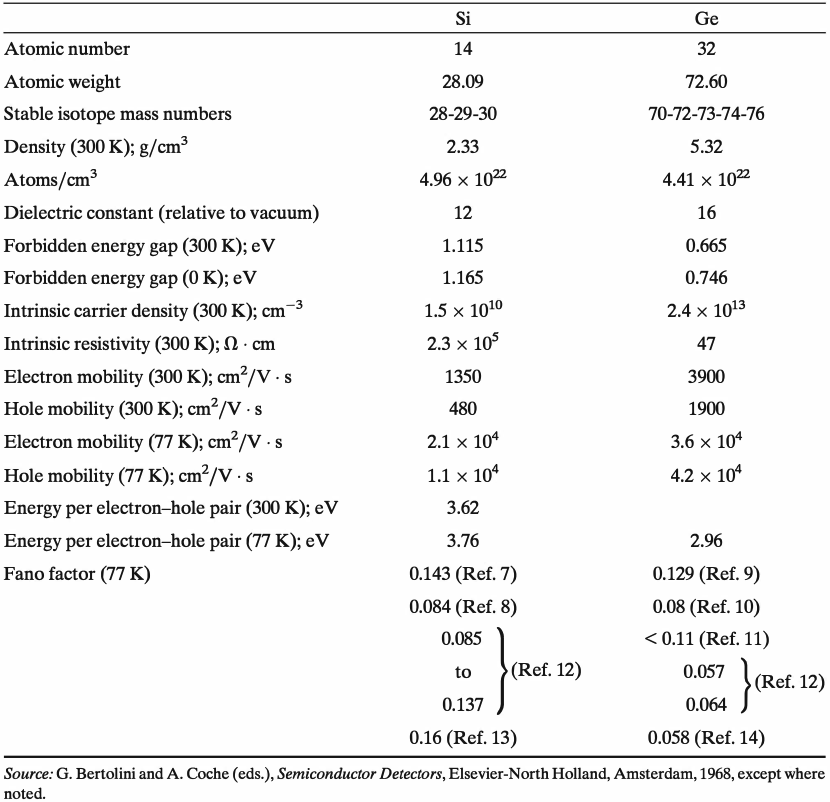
\includegraphics[width=1.0\textwidth]{images/Si_Ge_properties.png}
    \caption{Intrinsic properties of Si and Ge.}
    \label{fig:Si_Ge_properties}
\end{figure}
\subsubsection{Advantages or Semiconductor Detectors}
\begin{itemize}
    \item Good energy resolution due to small energy to generate information carriers (electron-hole pairs)
    \item High-density (solid)
    \item Good charge carrier collection properties
    \item Good timing characteristics
\end{itemize}
\subsubsection{Semiconductor vs. Gas Detectors}
\begin{itemize}
    \item Similarities:
    \begin{itemize}
        \item Ionization of detector material creating positive and negative charge carriers 
        \item Drift and collection of charge carriers due to external electric field
        \item Induction of signal during charge collection due to motion of charge carriers
    \end{itemize}
    \item Differences:\\
    A semiconductor detectors has
    \begin{itemize}
        \item Solid state counter with higher density and ($dE/dx$)
        \item Smaller energy to generate charge carriers
        \item Higher mobility
        \item Both types of charge carriers are fast
    \end{itemize}
\end{itemize}
\subsection{Principles of Operation}
\subsubsection{Band Gap and Ionization Energy}
\begin{figure}[ht]
    \centering
    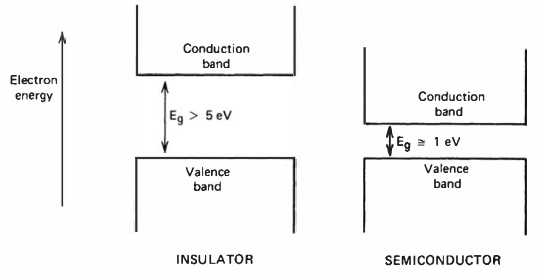
\includegraphics[width=0.5\textwidth]{images/semiconductor_band_structure.png}
    \caption{Band structure for insulators and semiconductors.}
    \label{fig:semiconductor_band_structure}
\end{figure}
\begin{itemize}
    \item In band theory, the energy of any electron within the pure material is confined to allowed energy bands, which may be separated by gaps or ranges of forbidden energies. As shown in figure~\ref{fig:semiconductor_band_structure}, the valence band corresponds to outer-shell electrons that are bound to specific lattice sites within the crystal; the conduction band represents electrons that migrate freely through the crystal. The band gap separates the two bands.
    \item Excitations in the crystal, where a valence electron gains sufficient energy to be elevated across the band gap into the conduction band, creates an electron-hole pair, analogous to a ion pair in gases. Ionizing radiation creates electron-hole pairs in the semiconductor as charge and information carriers. 
    \item As shown in the table below, the ratio of W to band gap is approximately constant for a wide range of materials, reflecting the constant ratio between electron-hole generation and phonon generation. See figure~\ref{fig:Si_Ge_properties} for more detailed Si and Ge intrinsic properties.
    \begin{center}
        \begin{tabular}{|c|c|c|c|}
        \hline
         &  Mean Ionization Energy W (eV) & Density (g/cm$^3$) & Fano Factor \\
        \hline
        Gases     & 30 & $7\sim50\times10^{-4}$ & $0.1\sim0.2$ (ionization vs. excitation)\\
        \hline
        Si & 3.62 & 2.33 & $\sim0.10$ (ionization vs. phonons)\\
        \hline
        Ge & 2.96 & 5.32 & $\sim0.10$ (ionization vs. phonons)\\
        \hline
        \end{tabular}
    \end{center}
\end{itemize}
\subsubsection{Lattice, Intrinsic Carrier Density,  Mobility, and Resistivity}
\begin{itemize}
    \item Lattice:\\
    Both Ge and Si have the diamond cubic crystal structure.
    \item Intrinsic carrier density:\\
    The intrinsic (no dopant) carrier density in a semiconductor is low.
    \begin{itemize}
        \item[] Assuming equilibrium between thermal excitation and recombination, 
        \item[] the concentration of electrons (or holes) $n_i=\sqrt{N_CN_V}\exp(-E_{Gap}/2k_BT)$
        \item[] , where $N_V$ and $N_C$ are the densities of states in the valence and conduction bands.
        \item[] Typical values of $n_i$ are $2.5\times10^{13}$ cm$^{-3}$ for Ge and $1.4\times10^{10}$ cm$^{-3}$ for Si.
        \item[] However, for example in Si, the atomic density $n_{atoms}=\frac{N_A\rho}{M}\approx5\times10^{22}\;\text{cm}^{-3}$
        \item[] Therefore, $f=(1.5\times10^{10})/(5\times10^{22})=3\times10^{-13}$ 
    \end{itemize}
    \item Mobility ($\mu$) and resistivity ($\rho$):
    \begin{itemize}
        \item[] The drift velocity is given by $v_{e/h}=\mu_{e/h}E$
        \item[] Current density $J=\text{charge density}\times v=en_i(\mu_e+\mu_h)E$
        \item[] Since $J=\sigma E$ where $\sigma$ is conductivity,
        \item[] $\rho=1/\sigma=[en_i(\mu_e+\mu_h)]^{-1}$
        \item[] Assuming only thermal excitations, where $n_i=n_p=n_e$, 
        \item[] with $n_i=10^{10}\;cm^{-3}$ and $\mu_e=1500\;cm^2/Vs$, then $\rho\sim10^5\;\Omega\cdot cm$
    \end{itemize}
\end{itemize}
\subsubsection{Doped Semiconductors}
\begin{itemize}
    \item n-type:\\
    Doped with group V elements (donors), the current is mainly due to excess electrons
    \item p-type:\\
    Doped with group III elements (acceptors), the current is mainly due to excess holes
    \item p-n junction:\\
    A depleted (charge carrier free) zone can be created by combining n and p regions to form a p-n junction due to charge carrier diffusion. The electric field or contact potential caused by the new space charges stop the diffusion. See figure~\ref{fig:pn_junction_formation} for visualization of the process.
    \begin{figure}[ht]
        \centering
        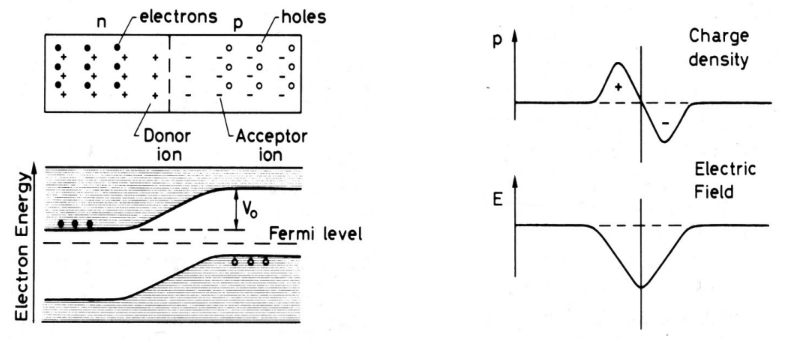
\includegraphics[width=0.5\textwidth]{images/pn_junction_formation.png}
        \caption{p-n junction formed due to charge carrier diffusion.}
        \label{fig:pn_junction_formation}
    \end{figure}
    \item Reverse-biased diode:\\
    By applying reverse bias, the depleted region of the p-n junction increases. See figure~\ref{fig:reverse_bias_diode}. 
    \begin{figure}[ht]
        \centering
        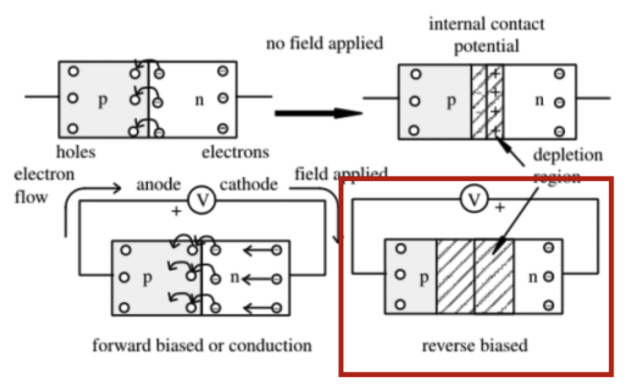
\includegraphics[width=0.5\textwidth]{images/reverse_bias_diode.png}
        \caption{Reverse-biasing of a diode.}
        \label{fig:reverse_bias_diode}
    \end{figure}
\end{itemize}
\subsubsection{Depletion Layer}
\begin{itemize}
    \item Depletion depth of a idealized junction (see figure~\ref{fig:depletion_depth_calc}):
    \begin{figure}[ht]
        \centering
        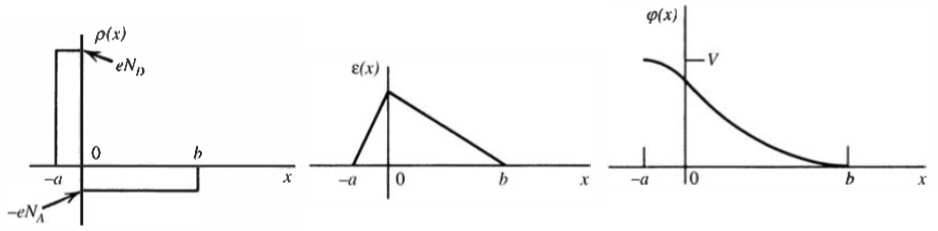
\includegraphics[width=0.8\textwidth]{images/depletion_depth_calc.png}
        \caption{Charge distribution (left), electric field (center), and potential (right) of a idealized junction.}
        \label{fig:depletion_depth_calc}
    \end{figure}
    \begin{itemize}
        \item In the idealized situation where the electron diffusion is assumed to result in a uniform positive space charge (ionized donor sites) over the region $-a<x\leq0$, and the hole diffusion results in a uniform negative space charge over the region $0\leq x<b$, 
        \begin{itemize}
            \item[] $\rho(x)=eN_D\;(-a<x\leq0)$
            \item[] $\rho(x)=eN_A\;(0<x\leq b)$
            \item[] $N_Da=N_Ab$ , due to charge neutrality
        \end{itemize}
        \item Poisson's equation states $\nabla^2\phi=-\rho/\epsilon$, where $\phi$ is the potential and $\epsilon$ is the dielectric constant of the material.
        \begin{itemize}
            \item[] $\frac{d^2\phi}{dx^2}=-\frac{eN_D}{\epsilon}\;(-a<x\leq0)$
            \item[] $\frac{d^2\phi}{dx^2}=+\frac{eN_A}{\epsilon}\;(0<x\leq b)$
        \end{itemize}
        \item With integration and the boundary condition that $E=-d\phi/dx=0$ at $x=-a$ and $x=b$,
        \begin{itemize}
            \item[] $\frac{d\phi}{dx}=-\frac{eN_D}{\epsilon}(x+a)\;(-a<x\leq0)$
            \item[] $\frac{d\phi}{dx}=+\frac{eN_A}{\epsilon}(x-b)\;(0<x\leq b)$
        \end{itemize}
        \item Further integration and boundary conditions of $\phi(-a)=V$ and $\phi(b)=0$ yields
        \begin{itemize}
            \item[] $\phi(x)=-\frac{eN_D}{2\epsilon}(x+a)^2+V\;(-a<x\leq0)$
            \item[] $\phi(x)=+\frac{eN_A}{2\epsilon}(x-b)^2\;(0<x\leq b)$
        \end{itemize}
        \item Since the above expressions of $\phi(x)$ has to match at $x=0$, with the condition given by charge neutrality,  
        \begin{itemize}
            \item[] $V-\frac{eN_D}{2\epsilon}(x+a)^2=\frac{eN_A}{2\epsilon}(x-b)^2$
            \item[] $(a+b)b=\frac{2\epsilon V}{eN_A}$
        \end{itemize}
        \item In this example, we assumed $N_D\gg N_A$, and hence $b\gg a$. Then $d\approx b$, and 
        \begin{itemize}
            \item[] $d\approx\left(\frac{2\epsilon V}{eN_A}\right)^{1/2}$
        \end{itemize}
        An opposite assumption would have given a identical result except that $N_A$ would be replaced $N_D$
        \item The generalized solution is therefore 
        \begin{itemize}
            \item[] $d\approx\left(\frac{2\epsilon V}{eN}\right)^{1/2}$
        \end{itemize}
        , where $N$ is the dopant concentration on the side of the junction that has the lower dopant level.
    \end{itemize}
    \item Characteristics of the depletion layer:
    \begin{itemize}
        \item Depletion voltage:\\
        The reverse bias voltage is increased to extend the depletion region across the entire thickness $T$ of the detector.\\
        $V_d={(eNT^2)}/{(2\epsilon)}$
        \item Operational voltage:\\
        The reverse bias voltage is further increased to above the depletion voltage to ensure full charge collection with sufficiently high electric fields across the depletion region.
    \end{itemize}
\end{itemize}
\subsection{Si Detectors}
\subsubsection{Varieties of Si Detectors}
\begin{itemize}
    \item Diffusion junction diodes:
    \begin{itemize}
        \item Junction formed by exposing a p-type material to a vapor of n-type impurity, which converts a region at the surface from a p-type material to a n-type material. For example, a n+ contact with Li or P diffusion at $\sim1000^\circ C$ on p-type material.
        \item Since the n-type surface layer is heavily doped compared with the p-type original crystal, the depletion region extends primarily into the p side of the junction. Much of the surface layer is therefore outside the depletion region, forming a dead layer. For the example given above, there would be a thick n+ dead layer.
        \item Carrier lifetime is reduced due to the high temperature process. 
        \item Earliest implementation, has been replaced in nearly all applications.
    \end{itemize}
    \item Silicon surface barrier (SSB) devices:
    \begin{itemize}
        \item Junction is formed between a semiconductor and certain metals. The depletion region behaves similar to that of the diffusion junction diode. 
        \item One production method is etching of the surface of n-type Si, followed by evaporation of a thin Au layer for electrical contact. Better results are obtained if slight oxidation occurs and an oxide layer is created between the Au and Si.
        \item Another method is to start with a p-type crystal and evaporate Al to form a n-type contact. 
        \item Very thin dead layer; the thickness can be measured by measuring the energy loss of particles within this layer. 
        \item Sensitive to light; the energy of visible photons is 2$\sim$4 eV, larger than the band gap.
    \end{itemize}
    \item Ion-implanted diodes:
    \begin{itemize}
        \item An alternative method of introducing doping impurities at the surface of the semiconductor is to expose that surface to a beam of ions produced by an accelerator. 
        \item A n+ contact can be formed by P implantation, and a p+ contact can be formed by B implantation.
        \item The annealing temperature is $\sim500^\circ C$; the crystal is less disturbed and carrier lifetimes are not necessarily reduced. 
        \item Very thin entrance window
    \end{itemize}
\end{itemize}
\subsubsection{Si(Li) Detectors}
\begin{figure}[ht]
    \centering
    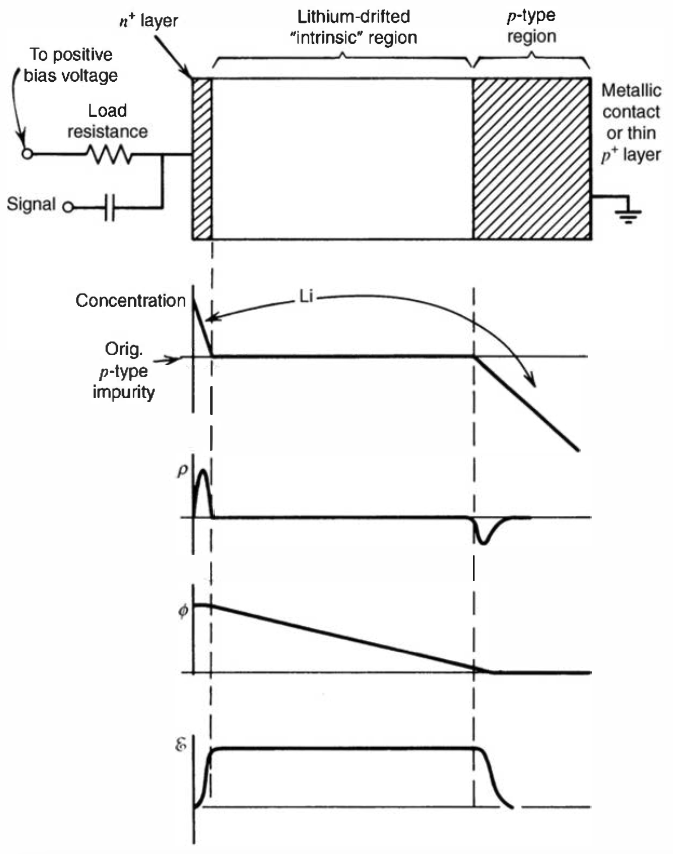
\includegraphics[width=0.5\textwidth]{images/SiLi_Detector.png}
    \caption{Configuration of a Si(Li) detector.}
    \label{fig:SiLi_Detector}
\end{figure}
\begin{itemize}
    \item Intrinsic high-purity Si detectors have limited thickness of $<2$ mm due to a minimum impurity concentration of $\sim10^{12}\;\text{cm}^{-3}$ (due to the crystal growth process) and a maximum applicable voltage of $<2000$ V (leakage current degrades energy resolution). 
    \item Li-drifting in p-type Si compensates the impurities. 
\end{itemize}
\subsubsection{Si Detector Applications}
\begin{itemize}
    \item Position-sensitive Si detectors:\\
    Strip-detectors, micro-strip detectors, Si-drift detectors (good energy resolution at room temperature), circular Si-drift detectors (high energy resolution)
    \item $\alpha$-particle spectroscopy
    \item Conversion electron spectroscopy and counting
    \item X-ray spectroscopy, fluorescence, or imaging
    \item Charged particle timing, energy measurement, and identification ($\Delta$E-E telescope)
\end{itemize}

\subsection{Ge Detectors}
\subsubsection{Overview}
\subsubsection{Planar and Coaxial Configurations}
\subsubsection{Energy Spectra and Efficiency}
\subsubsection{Varieties of Ge Detectors}

\subsection{Alternative Semiconductor Detectors}
\subsubsection{Limitations of Ge Detector Operations}
\subsubsection{Lifetime and Mobility}
\subsubsection{Charge Collection Properties}